% ABC Vehicraft. IEEE ICCE 2027 (Las Vegas), IEEE conference template.
% Draft for co-authors. Red [TODO] marks are open.
\documentclass[conference]{IEEEtran}
\IEEEoverridecommandlockouts
\usepackage{cite}
\usepackage{amsmath,amssymb}
\usepackage{graphicx}
\usepackage{booktabs}
\usepackage{xcolor}
\usepackage{url}
\usepackage[hidelinks]{hyperref}
\graphicspath{{figures/}}

\newcommand{\todo}[1]{\textcolor{red}{[TODO: #1]}}

\begin{document}

\title{ABC Vehicraft: The Aerial Boat Car, and What a Consumer EEG Headband Records While Riding It}

\author{
\IEEEauthorblockN{Alexander Vicol and Steve Mann}
\IEEEauthorblockA{University of Toronto and MannLab Canada, Toronto, Canada\\
vicola.lexo@gmail.com}
}

\maketitle

\begin{abstract}
We introduce the ABC Vehicraft, a craft that is at once aerial, boat and car, and report the first brain-sensing recordings taken while riding it. On one afternoon in Toronto's harbour the second author rode three modes of the craft wearing a Muse S Athena headband streaming to a phone: standing on a paddle board, walking inside a water-walking ball, and lying on a board with the ears at the waterline. No headset, no laptop, no marker, 3.6 to 4.9 minutes per mode. We ask what such a recording is good for. The paddle board gives usable EEG on 88\% of 2\,s epochs behind the ears and 98\% on the left forehead; the ball halves that and the board in the water leaves one epoch in six behind the ears. The theta/beta ratio, the attentional-control marker of our State-of-Float work, reads 2.7 on the paddle board, 1.6 on the board in the water, and 6.9 in the ball, where a 2.4\,Hz step rhythm in the accelerometer and a threefold rise in delta and theta say that the number is motion, not mind. The headband's own arousal index sat at 0.41, 0.49 and 0.47. The optical channels logged nothing, so there is no fNIRS. The paper's contribution is the craft and an honest account of what a wet, moving, open-air headband gives, with the recording rules that follow for the next ride: a strap over the band, dry ear sites, a logged fNIRS stream, a trigger per mode, and two-minute eyes-open and eyes-closed blocks in each.
\end{abstract}

\begin{IEEEkeywords}
Mersivity; wearable computing; EEG; brain-computer interface; consumer electronics; water-walking ball; paddle board; theta/beta ratio; amphibious vehicle; extended reality.
\end{IEEEkeywords}

\section{Introduction}

Mersivity is the idea that technology should connect people to each other and to the natural world rather than wall them off from it \cite{mann2026float}, and that wearable sensing \cite{mann1997wearable} lets the laboratory come out to the lake instead of bringing the lake's people into a laboratory. Our State-of-Float paper took a consumer EEG headband into a water-walking ball and found a higher theta/beta ratio while floating than on land \cite{mann2026float}. That work was done lying still under a VR headset, in two-minute blocks, with the headset pressing the headband into place.

This paper goes the other way. The craft moves, the rider stands, walks or swims, nothing presses the headband down, and the water reaches the electrodes. The question is what a consumer headband records under those conditions, because the answer decides whether brain-state measurement can travel with a vehicle at all. We do it on the ABC Vehicraft, a craft built to be aerial, boat and car at once, and we record its rider on three of its modes in one afternoon.

We make no claim about the rider's state from these recordings. Three to five minutes per mode, one person, no markers and no baseline is not a study of mind. It is a study of the measurement, and it yields a table of what each mode gives, which artifacts dominate, and what the next ride must add. That is the contribution, together with the craft itself.

\section{The ABC Vehicraft}

\todo{the concept and the engineering in the second author's words: what the aerial, boat and car elements are, how they combine, and what the craft is for}

Figs.~\ref{fig:photos} to~\ref{fig:ballsun} show the craft on October 9, 2026, in Toronto's inner harbour. The elements the pictures show: a stand-up paddle board, the boat; a helium balloon cluster tethered to the craft, the aerial element, which marks the craft from a distance and takes the first grams of its load into the air; and the water-walking ball, a transparent inflatable sphere two metres across that rolls on land and on water, the element that behaves like a wheel \cite{mann2026float, astm2374}. The rider wears a Muse S Athena headband throughout.

\begin{figure*}[t]
\centering
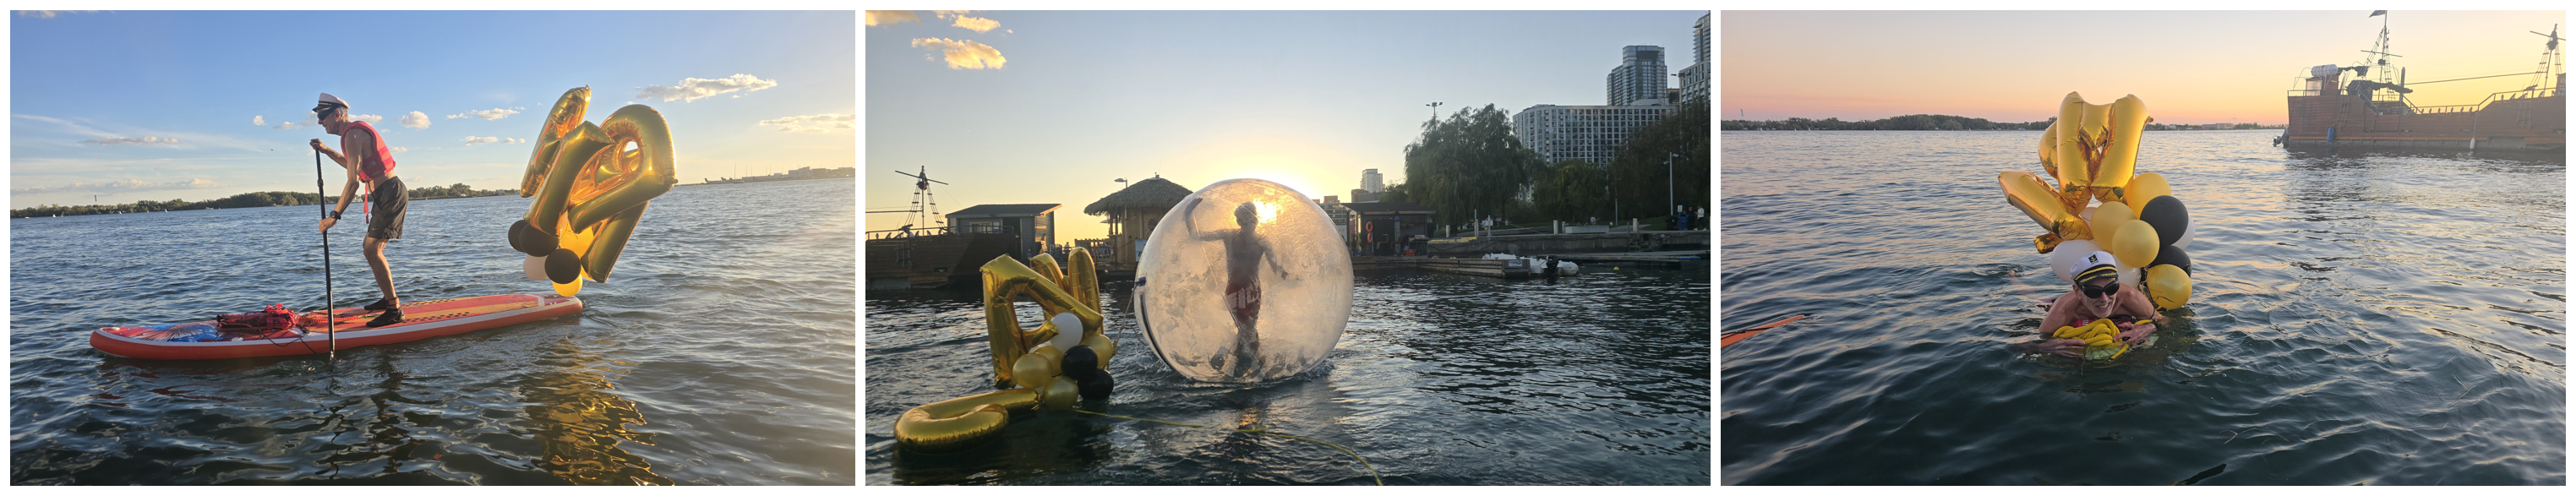
\includegraphics[width=0.9\textwidth]{photos}
\caption{The three modes of the ABC Vehicraft in Toronto's harbour, October 9, 2026, in the order they were recorded. Left: the paddle board under way with the balloon cluster in tow. Middle: the water-walking ball at sunset. Right: the Billy board, the small board ridden in the water with the ears at the waterline. The rider wears the Muse S Athena headband in every picture.}
\label{fig:photos}
\end{figure*}

\begin{figure}[t]
\centering
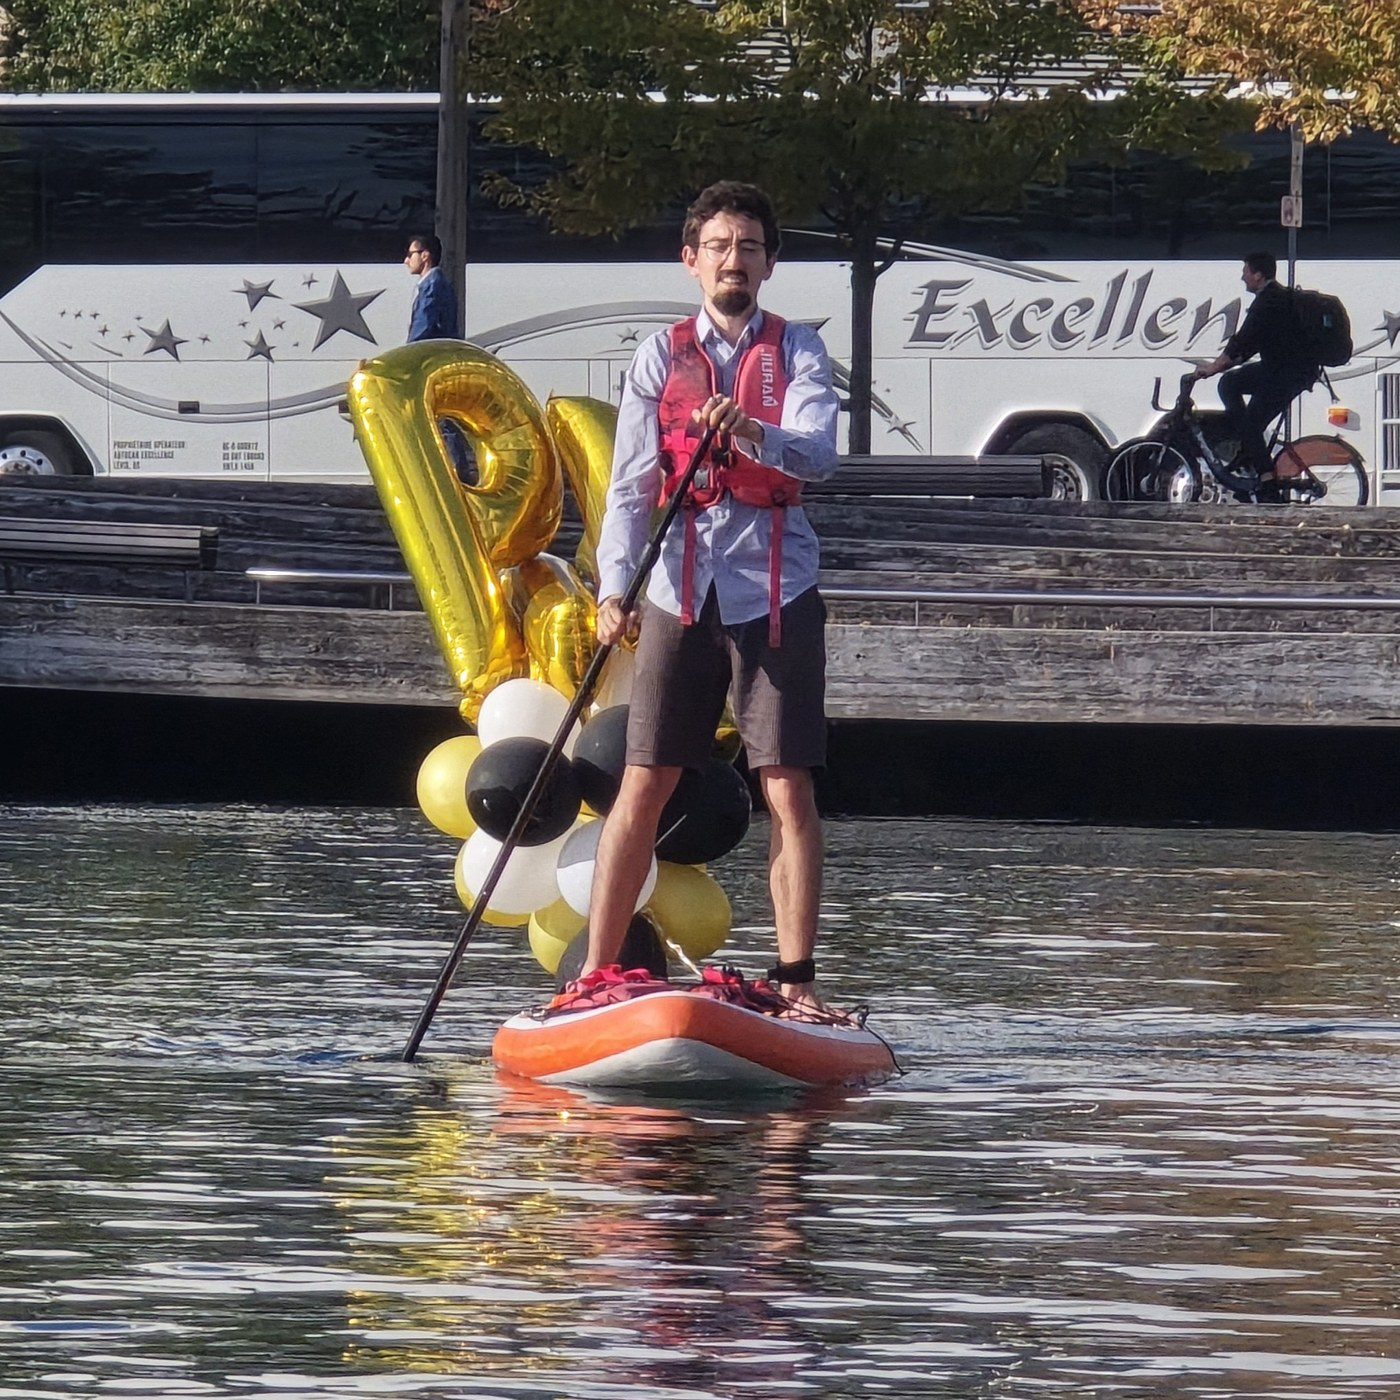
\includegraphics[width=0.78\columnwidth]{photo_second_rider}
\caption{The first author on the same craft earlier in the afternoon, the balloon cluster at the bow, in the inner harbour.}
\label{fig:second}
\end{figure}

\begin{figure}[t]
\centering
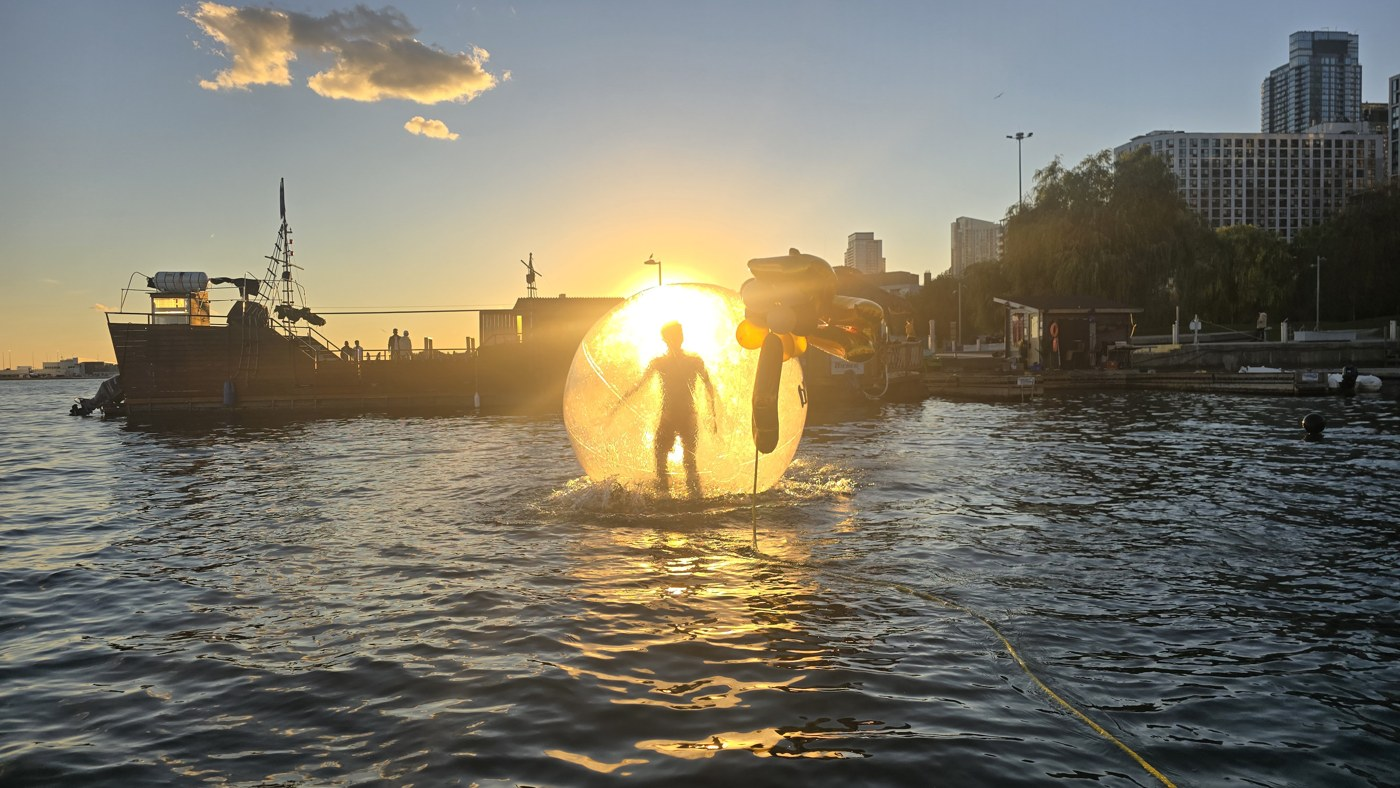
\includegraphics[width=\columnwidth]{photo_ball_sun}
\caption{The water-walking ball against the setting sun, with the balloon cluster tethered alongside and the tow line trailing to the camera.}
\label{fig:ballsun}
\end{figure}

Three modes were recorded, each as one continuous MuseLog file (Table~\ref{tab:modes}): standing and paddling on the board at 17:51, walking inside the ball at 18:16, and lying on the board in the water at 18:51, with the ears at or under the surface. \todo{the name and the construction of the third mode's board, recorded as the Billy board}

\section{Methods}

\textbf{Recording.} Muse S Athena, four dry EEG electrodes at TP9, AF7, AF8 and TP10 referenced at Fpz, 256\,Hz, streamed over Bluetooth to a phone running MuseLog, which writes one CSV row per sample with the raw channels, the headband's own band powers, head-set indicators, accelerometer and gyroscope, the optical channels, and the headband's arousal index. No headset, no laptop, no stimulus. The headband's fit indicator read 4, its poorest value, on every channel for the whole of every file; what that meant in practice is what the usable-epoch counts below measure. The optical columns (730 and 850\,nm, red and ambient, inner and outer, both sides) are empty in all three files: the fNIRS stream was not logged, so there is no fNIRS in this paper.

\textbf{EEG.} Raw channels band-passed 1 to 100\,Hz, cut into 2\,s epochs, an epoch usable when its peak stays under 200\,$\mu$V. Spectra are Welch estimates over the usable epochs (4\,s segments). Band powers are delta 1 to 4, theta 4 to 8, alpha 8 to 13, beta 13 to 30 and gamma 30 to 45\,Hz. The theta/beta ratio (TBR), the marker of our State-of-Float work and a marker of attentional control \cite{putman2010tbr, angelidis2016tbr}, is theta over beta per 10\,s window, the median over the four channels, usable windows only. We report the headband's arousal index per 10\,s as the device gives it.

\textbf{Motion.} The accelerometer magnitude's spectrum from 0.2 to 5\,Hz gives the dominant rhythm of the head; the gyroscope magnitude's median gives the rotation rate.

\begin{table}[t]
\caption{The three modes and what each recording gave. Usable epochs are 2\,s epochs under 200\,$\mu$V on the ear channels (TP9, TP10) and on AF7. TBR is the median theta/beta ratio over 10\,s windows. Rhythm is the accelerometer's dominant frequency.}
\label{tab:modes}
\centering
\scriptsize
\setlength{\tabcolsep}{4pt}
\begin{tabular}{lcccccc}
\toprule
mode & start & min & ears / AF7 usable & TBR & arousal & rhythm \\
\midrule
paddle board, standing & 17:51 & 4.9 & 88\% / 98\% & 2.7 & 0.41 & 2.3\,Hz \\
water ball, walking & 18:16 & 3.6 & 50\% / 72\% & 6.9 & 0.49 & 2.4\,Hz \\
board, ears in water & 18:51 & 3.6 & 16 to 33\% / 93\% & 1.6 & 0.47 & 1.05\,Hz \\
\bottomrule
\end{tabular}
\end{table}

\section{Results}

\textbf{Contact and artifact.} Fig.~\ref{fig:quality}. Standing on the paddle board the headband gave usable EEG on 88\% of epochs behind both ears and 98\% on the left forehead, at 30\,$\mu$V rms behind the ears and 16 on AF7, numbers a quiet indoor session would not be ashamed of. The right forehead electrode (AF8) was off the skin in every mode, 11 to 22\% usable, and is dropped from what follows. Walking in the ball halved the usable share behind the ears to 50\% and on AF7 to 72\%, with rms up by a third. With the ears in the water the ear electrodes gave one usable epoch in three on the left and one in six on the right, at 46\,$\mu$V, while AF7, above the waterline, stayed 93\% usable.

\begin{figure}[t]
\centering
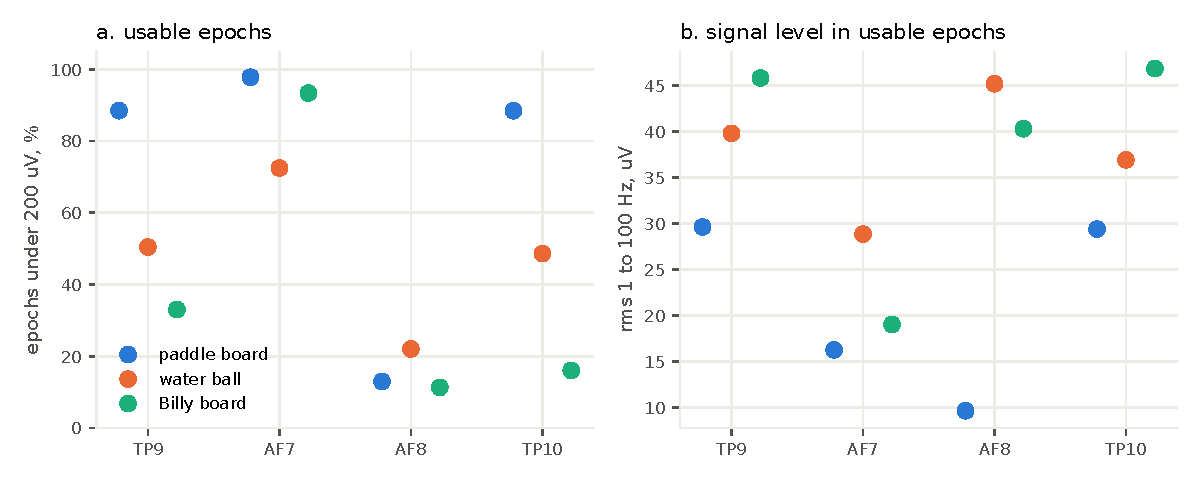
\includegraphics[width=\columnwidth]{fig_quality}
\caption{What each mode gives per electrode: the share of 2\,s epochs under 200\,$\mu$V (left) and the rms of the usable epochs (right).}
\label{fig:quality}
\end{figure}

\textbf{Spectra.} Fig.~\ref{fig:spectra}. Behind the left ear the paddle board's spectrum is the ordinary 1/f shape with an alpha shoulder near 10\,Hz. The ball raises the whole spectrum by a factor of two to three and the low end by more. The board in the water raises everything above 10\,Hz by a factor of three to four with a broad hump at 12 to 16\,Hz, the signature of water and muscle at the ear site rather than cortex. On the forehead the three modes differ mainly below 10\,Hz, where the ball's walking rhythm and its harmonics sit.

\begin{figure}[t]
\centering
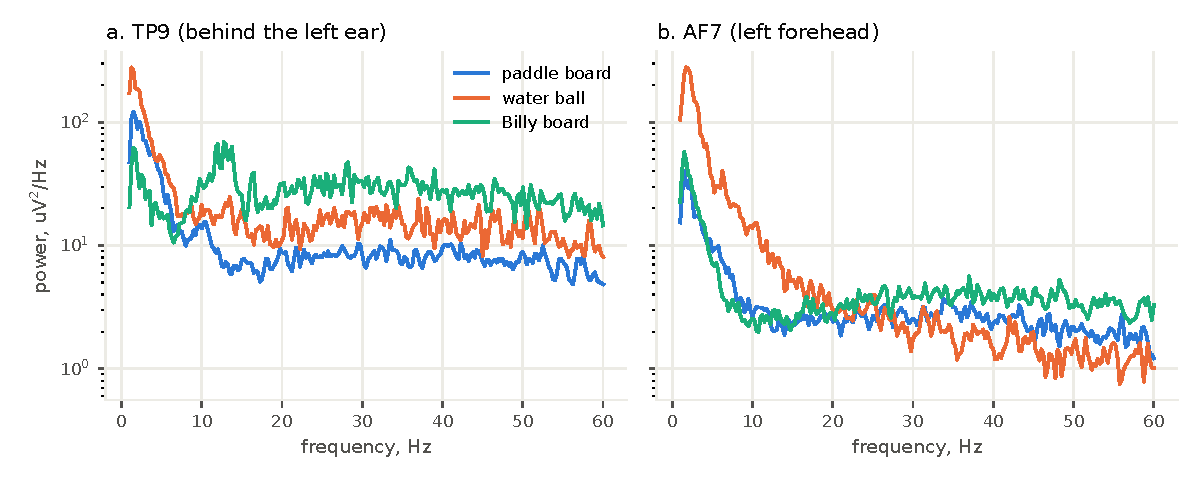
\includegraphics[width=\columnwidth]{fig_spectra}
\caption{Power spectra of the usable epochs, behind the left ear (left) and on the left forehead (right), one line per mode.}
\label{fig:spectra}
\end{figure}

\textbf{Band powers and the theta/beta ratio.} Fig.~\ref{fig:bands}. On the ear channels the paddle board sits lowest in every band. The ball more than doubles delta and theta while adding less to beta, which is why its TBR is 6.9 against the paddle board's 2.7; the board in the water adds most to alpha, beta and gamma, which is why its TBR is lowest at 1.6. Read as brain state these would be a calmer rider in the ball and an aroused one in the water. Read with the motion and contact figures they are the opposite of a finding: delta and theta inflated by a 2.4\,Hz step rhythm and its harmonics in the ball, and beta and gamma inflated by water and muscle at the ear sites on the board. The TBR of the paddle board, the one mode where the electrodes held and the head moved little, is the only one of the three we would quote, and it is in the range our floating subjects gave on land \cite{mann2026float}.

\begin{figure}[t]
\centering
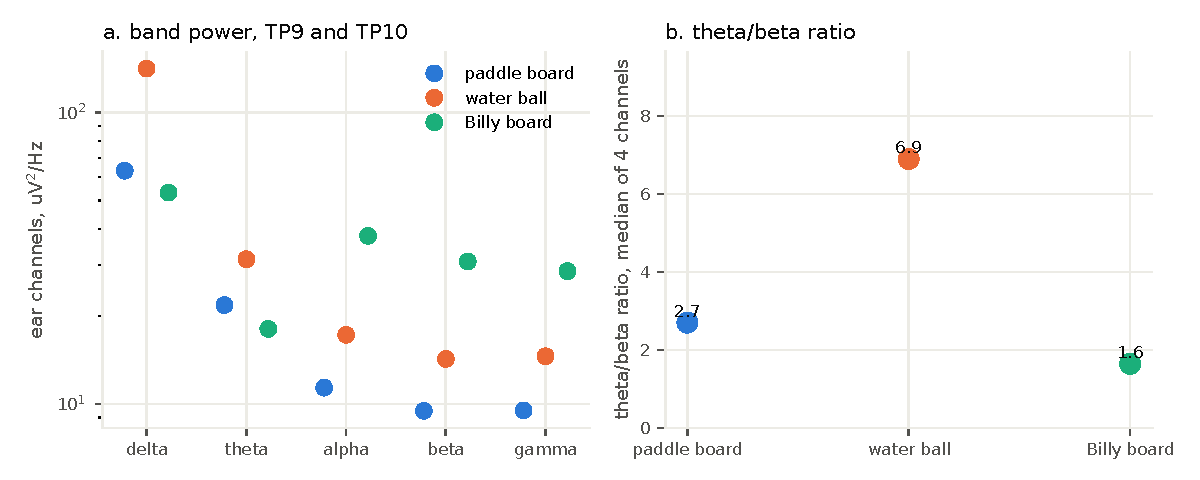
\includegraphics[width=\columnwidth]{fig_bands}
\caption{Band power on the ear channels (left) and the theta/beta ratio (right) per mode. The ball's ratio is carried by motion-inflated delta and theta, the water board's low ratio by water and muscle in the beta band.}
\label{fig:bands}
\end{figure}

\textbf{Motion.} Fig.~\ref{fig:motion}. The accelerometer shows the rider's rhythm on each craft: a sharp 2.4\,Hz line in the ball, which is the step rate of walking on a surface that rolls away underfoot, at a head-acceleration spread of 0.16\,g and a median rotation rate of 22 degrees per second; a 2.3\,Hz rhythm on the paddle board at 0.06\,g, the board's chop and the paddle's cadence; and a 1.05\,Hz rhythm on the board in the water at 0.07\,g, the swimming stroke. The step line in the ball sits inside the delta band's second harmonic and the theta band's third, which is where its EEG excess appears.

\begin{figure}[t]
\centering
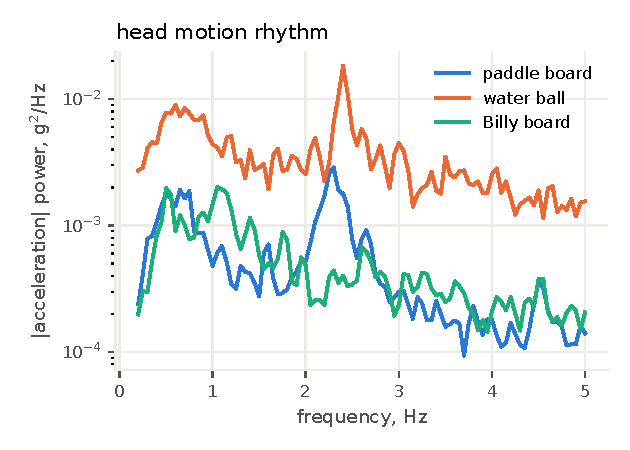
\includegraphics[width=0.8\columnwidth]{fig_motion}
\caption{Head-motion spectra from the headband's accelerometer. The ball's 2.4\,Hz line is the rider's step rate.}
\label{fig:motion}
\end{figure}

\textbf{Through each ride.} Fig.~\ref{fig:course}. On the paddle board the TBR falls through the first two minutes from 9 to about 2 and stays there, the pattern of a headband settling after it is put on wet rather than of a mind changing; the headband's arousal index is live for the first 1.7 minutes and then holds a constant 0.3, which is the device's output when it stops updating, not a reading. In the ball the TBR is measurable only in the usable windows and ranges from 2 to 17, and the arousal index swings between 0.1 and 0.85 with the rider's bouts of walking and standing. On the board in the water the TBR settles from 5 to between 1 and 3 and the arousal index, available only from the second minute, sits at 0.3 to 0.7.

\begin{figure}[t]
\centering
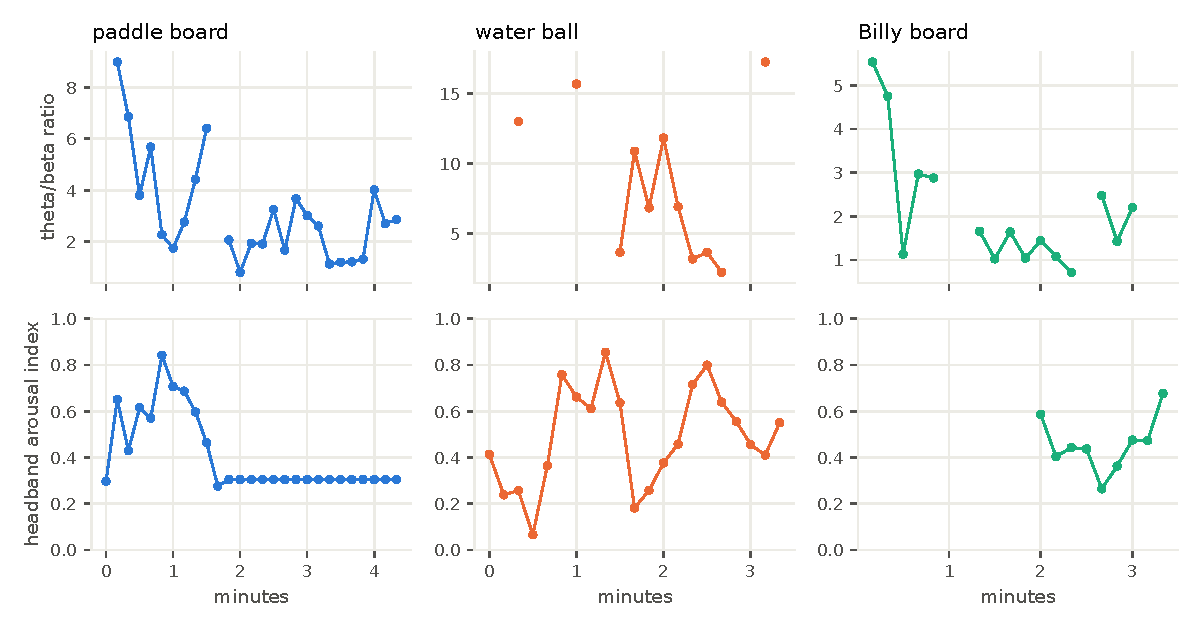
\includegraphics[width=\columnwidth]{fig_timecourse}
\caption{The theta/beta ratio (top) and the headband's arousal index (bottom) per 10\,s through each ride. Gaps are windows without a usable channel.}
\label{fig:course}
\end{figure}

\section{What It Means}

\textbf{Which modes can be measured.} Standing on a paddle board is a measurable condition for a consumer headband with nothing holding it down: nine epochs in ten usable behind the ears and the forehead nearly clean. Walking in the ball is a motion condition first and a brain condition second; its band powers are not interpretable without a motion model, and the honest number from it is the step rate. Ears in the water is not a condition the ear electrodes survive, though the forehead does, so a frontal-only analysis is possible there and an ear-based one is not.

\textbf{Rules for the next ride.} A strap or cap over the headband, which in our headset work improved contact by pressing the band in \cite{mann2026float}. Dry the ear sites and keep them above the waterline when the ear channels matter. Log the optical stream: the Athena's fNIRS is the one signal that does not care about a wet electrode, and it was not recorded. A trigger press at the start of each mode and each change of activity, so the file carries its own timeline. Two-minute eyes-open and eyes-closed blocks in each mode, still, as in the State-of-Float protocol, so that the TBR has the baseline it needs. And a reference recording on land the same day. With those, the same afternoon becomes the study this paper is not.

\textbf{Limits.} One rider, one afternoon, three to five minutes per mode, no markers, no baseline, no fNIRS. The fit indicator read its poorest value throughout, so the usable-epoch rule is the only guard on contact. The arousal index is the device's own and its algorithm is not published. Nothing here says what riding the craft does to a mind; it says what the headband can see while a mind rides it.

\section{Conclusion}

The ABC Vehicraft is a craft that is aerial, boat and car, and a vessel for brain-state measurement in the natural world. Its first ride with a consumer headband shows which of its modes a wet, moving, unpressed headband can measure. The paddle board, yes, with usable EEG on nine epochs in ten. The ball, as motion, with a step rate the accelerometer reads cleanly and EEG bands it inflates. The water, on the forehead only. The theta/beta ratio read 2.7 on the board, in the range of our earlier floating work, and the other two ratios are motion and water rather than mind. The next ride carries a strap, a trigger, the fNIRS stream and the two-minute blocks, and then the question changes from whether the craft can be measured to what it does to the rider.

\section*{Acknowledgements}
\todo{MannLab Canada; the harbour crew; Interaxon. Confirm wording.}

\bibliographystyle{IEEEtran}
\bibliography{refs}

\end{document}
